\newpage
\setcounter{subsection}{0}
\section{DESARROLLO DE LA SOLUCIÓN}

Esta sección describe el proceso seguido para materializar el diseño en un prototipo operativo sobre \textit{testnet}. La metodología combinó cuatro fases articuladas: revisión técnica, diseño de arquitectura, implementación incremental y evaluación experimental, ejecutadas bajo un esquema ágil con tablero Kanban y revisiones semanales con el director del trabajo de grado. El detalle de la planeación se documenta en el anexo SPMP.

\subsection{Implementación de contratos Soroban}

Los contratos se desarrollan en Rust contra \texttt{soroban-sdk} versión 23, organizados como un Cargo \textit{workspace} con tres paquetes: \texttt{event\_contract}, \texttt{factory\_contract} y \texttt{ticket\_nft\_contract}. El perfil de compilación \texttt{release} aplica \texttt{opt-level="z"}, \textit{Link-Time Optimization}, eliminación de símbolos y \texttt{panic="abort"}, lo que produce módulos WASM compatibles con el target \texttt{wasm32v1-none}.

El contrato \texttt{event\_contract} comprende aproximadamente 1\,142 líneas de código fuente en \texttt{lib.rs} y 709 líneas de pruebas en \texttt{test.rs}, con 35 casos unitarios. El contrato \texttt{factory\_contract} comprende 431 líneas de código y 245 de pruebas, con 13 casos. El contrato \texttt{ticket\_nft\_contract} (introducido en la fase 4.5 del proyecto, estilo SEP-41) ocupa aproximadamente 12\,KB de WASM y agrega 10 casos. El total de pruebas automatizadas es de 58 casos, ejecutables mediante \texttt{cargo test} en el \textit{workspace}.

\subsubsection{NFT del boleto: emisión, propiedad y versionado}

El boleto se modela bajo la estructura \texttt{Boleto} y la clave de almacenamiento \texttt{ClaveDato::Boleto(u32, u32)}, donde la tupla corresponde a \((\texttt{ticket\_root\_id}, \texttt{version})\). La asignación del \texttt{ticket\_root\_id} se realiza en \texttt{crear\_boleto} mediante el contador \texttt{ContadorBoletos}, que se incrementa atómicamente por cada emisión. Cada cambio de propiedad en reventa incrementa \texttt{version} y actualiza el puntero \texttt{VersionActual(ticket\_root\_id)}.

\subsubsection{Pagos atómicos vía SAC}

El activo de pago utilizado es XLM expuesto vía \textit{Stellar Asset Contract} (SAC). La transferencia se realiza mediante invocación al método \texttt{transfer} del SAC dentro del mismo \textit{call frame} de \texttt{comprar\_boleto}, lo que garantiza que el pago, la distribución de comisiones y el cambio de propiedad ocupen una única transacción del ledger. La Figura~\ref{fig:seq-reventa} muestra el diagrama de secuencia del flujo crítico de compra en reventa atómica.

\begin{figure}[H]
\centering
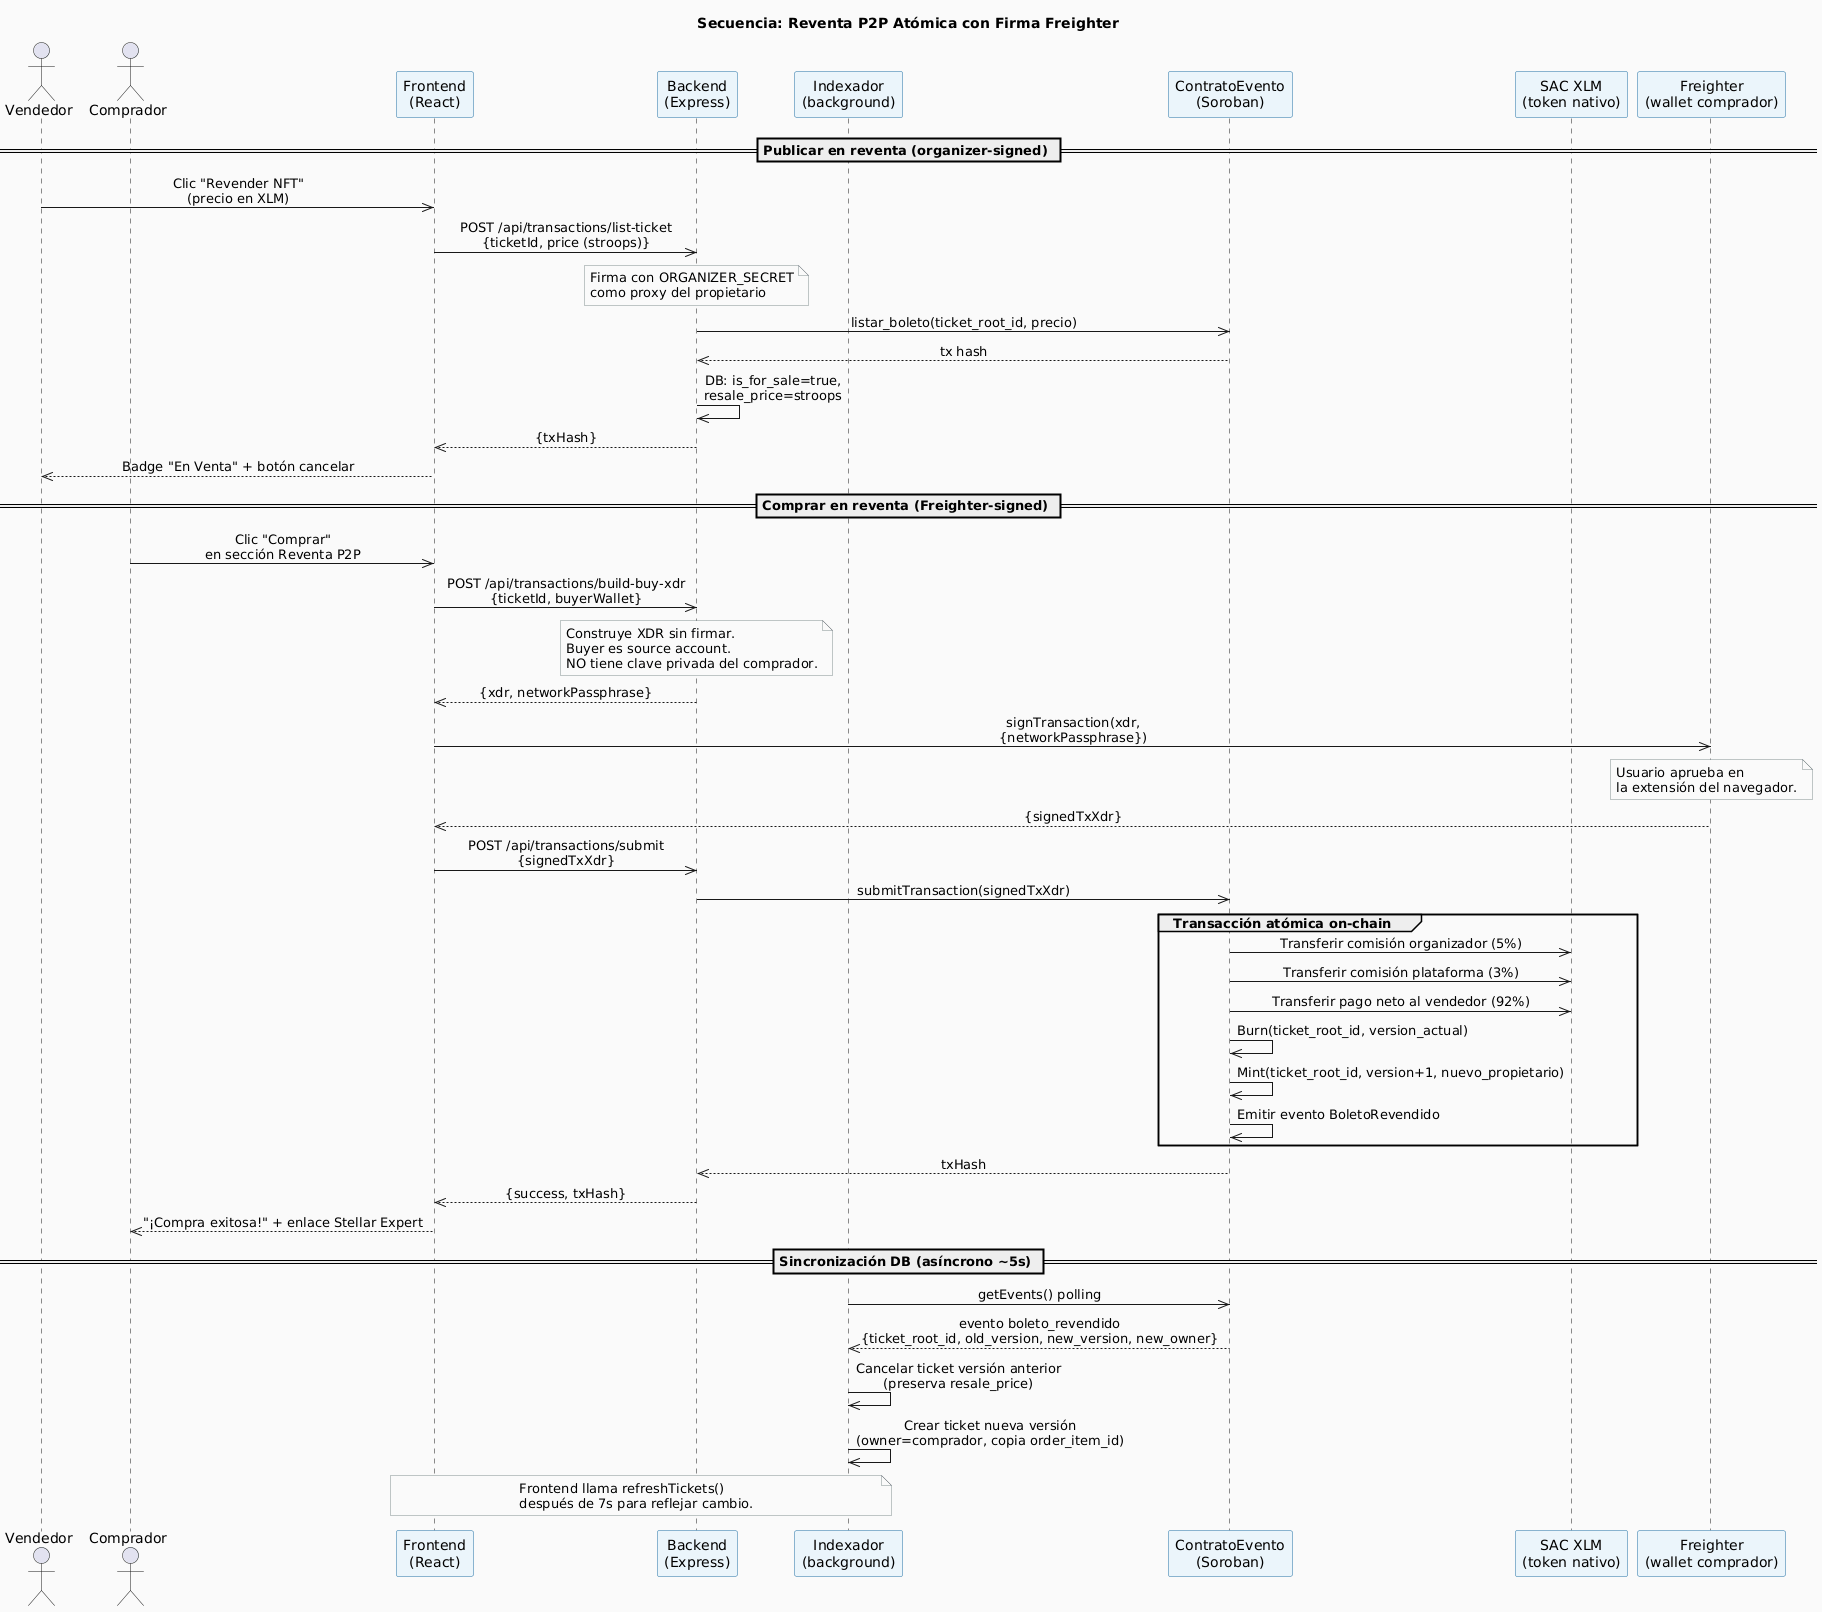
\includegraphics[width=\textwidth]{Imagenes/04_secuencia_reventa_atomica.png}
\caption{Diagrama de secuencia: compra en reventa atómica (pago al vendedor, comisión a organizador y plataforma, \textit{burn} de la versión vigente y \textit{remint} de la nueva, todo en una sola transacción).}
\label{fig:seq-reventa}
\end{figure}

\subsubsection{Redención y control de acceso}

La redención se controla mediante el rol verificador. El organizador registra direcciones autorizadas con \texttt{agregar\_verificador} y las remueve con \texttt{remover\_verificador}. La operación \texttt{redimir\_boleto} valida la pertenencia con \texttt{es\_verificador}, marca \texttt{usado=true} y emite el evento correspondiente. En el prototipo, el flujo en puerta opera contra la base de datos relacional para minimizar la latencia frente al usuario final, y la invocación on-chain se reserva para auditoría posterior. La Figura~\ref{fig:seq-verificacion} resume la secuencia.

\begin{figure}[H]
\centering
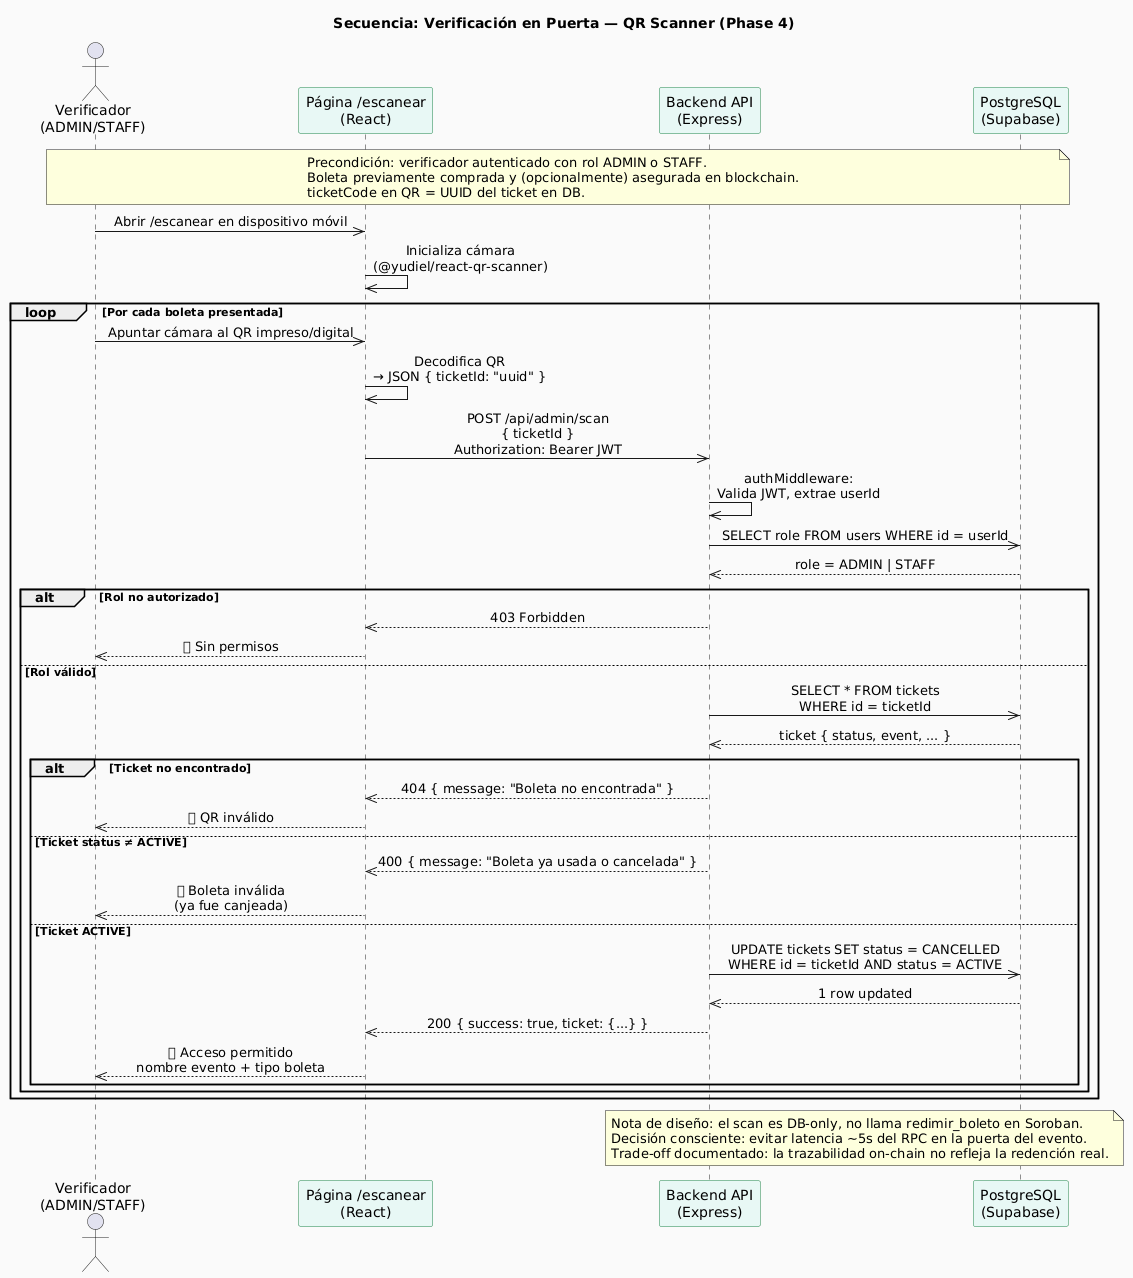
\includegraphics[width=0.95\textwidth]{Imagenes/05_secuencia_verificacion_puerta.png}
\caption{Diagrama de secuencia: verificación del boleto en puerta (escaneo QR, validación en PostgreSQL y respaldo on-chain).}
\label{fig:seq-verificacion}
\end{figure}

\subsection{Backend Node.js + Stellar SDK}

El backend está implementado en Node.js con Express, TypeScript y Prisma como ORM. Las dependencias principales son \texttt{express}, \texttt{@prisma/client}, \texttt{@stellar/stellar-sdk} (14.4.1), \texttt{cors}, \texttt{dotenv}, \texttt{bcryptjs} y \texttt{jsonwebtoken}. Las variables de entorno requeridas son \texttt{DATABASE\_URL}, \texttt{SOROBAN\_RPC\_URL}, \texttt{HORIZON\_URL}, \texttt{PORT}, \texttt{JWT\_SECRET}, \texttt{ORGANIZER\_SECRET} y \texttt{FACTORY\_CONTRACT\_ID}.

\subsubsection{API: usuarios, eventos, carrito, checkout y Soroban}

La API expone seis familias de endpoints: catálogo público con caché en memoria; autenticación con \texttt{bcrypt} y JWT; carrito con aislamiento por \texttt{user\_id}; \textit{checkout} fiat transaccional (creación de \texttt{orders}, \texttt{order\_items}, \texttt{tickets} y \texttt{payments} en una transacción Prisma atómica); integración Soroban (\texttt{secure-ticket}, \texttt{list-ticket}, \texttt{cancel-listing}, \texttt{build-buy-xdr}, \texttt{submit}); y la cadena de coleccionable Stellar Classic. Adicionalmente expone endpoints de administración (\texttt{GET/POST /api/admin/events}, \texttt{POST /api/admin/events/:id/deploy}, \texttt{POST /api/admin/scan}).

\subsubsection{Indexador: ingesta de eventos}

El indexador (\texttt{src/indexer.ts}) consulta Soroban RPC cada 5 segundos. Mantiene cursor en \texttt{indexer\_state.last\_ledger} con valor inicial 100 ledgers atrás. Procesa eventos en \textit{chunks} de hasta 1\,000 ledgers por solicitud y agrupa hasta cinco direcciones de contrato por filtro. Cada evento tiene un manejador idempotente: la verificación de existencia previa ante \texttt{boleto\_revendido} evita conflictos por reentrega; el manejador P2P preserva el campo \texttt{order\_item\_id} entre versiones. Ante errores transitorios el indexador reintenta tras 5 segundos; si el cursor cae fuera de la ventana de retención del RPC, parsea el error y se reposiciona al mínimo permitido.

\subsubsection{Persistencia: historial, listados y auditoría}

El esquema relacional Prisma define los enumerados \texttt{user\_role}, \texttt{event\_status}, \texttt{cart\_status}, \texttt{order\_status}, \texttt{payment\_method}, \texttt{payment\_status}, \texttt{seat\_inventory\_status}, \texttt{ticket\_status} y \texttt{venue\_type}. Los campos Web3 añadidos al modelo \texttt{tickets} (\texttt{contract\_address}, \texttt{ticket\_root\_id}, \texttt{version}, \texttt{is\_for\_sale}, \texttt{resale\_price}, \texttt{owner\_wallet}, \texttt{asset\_code}) y el índice único \((\texttt{contract\_address}, \texttt{ticket\_root\_id}, \texttt{version})\) reflejan la unicidad on-chain en el plano relacional. La Figura~\ref{fig:erd} muestra el modelo entidad-relación de la capa off-chain.

\begin{figure}[H]
\centering
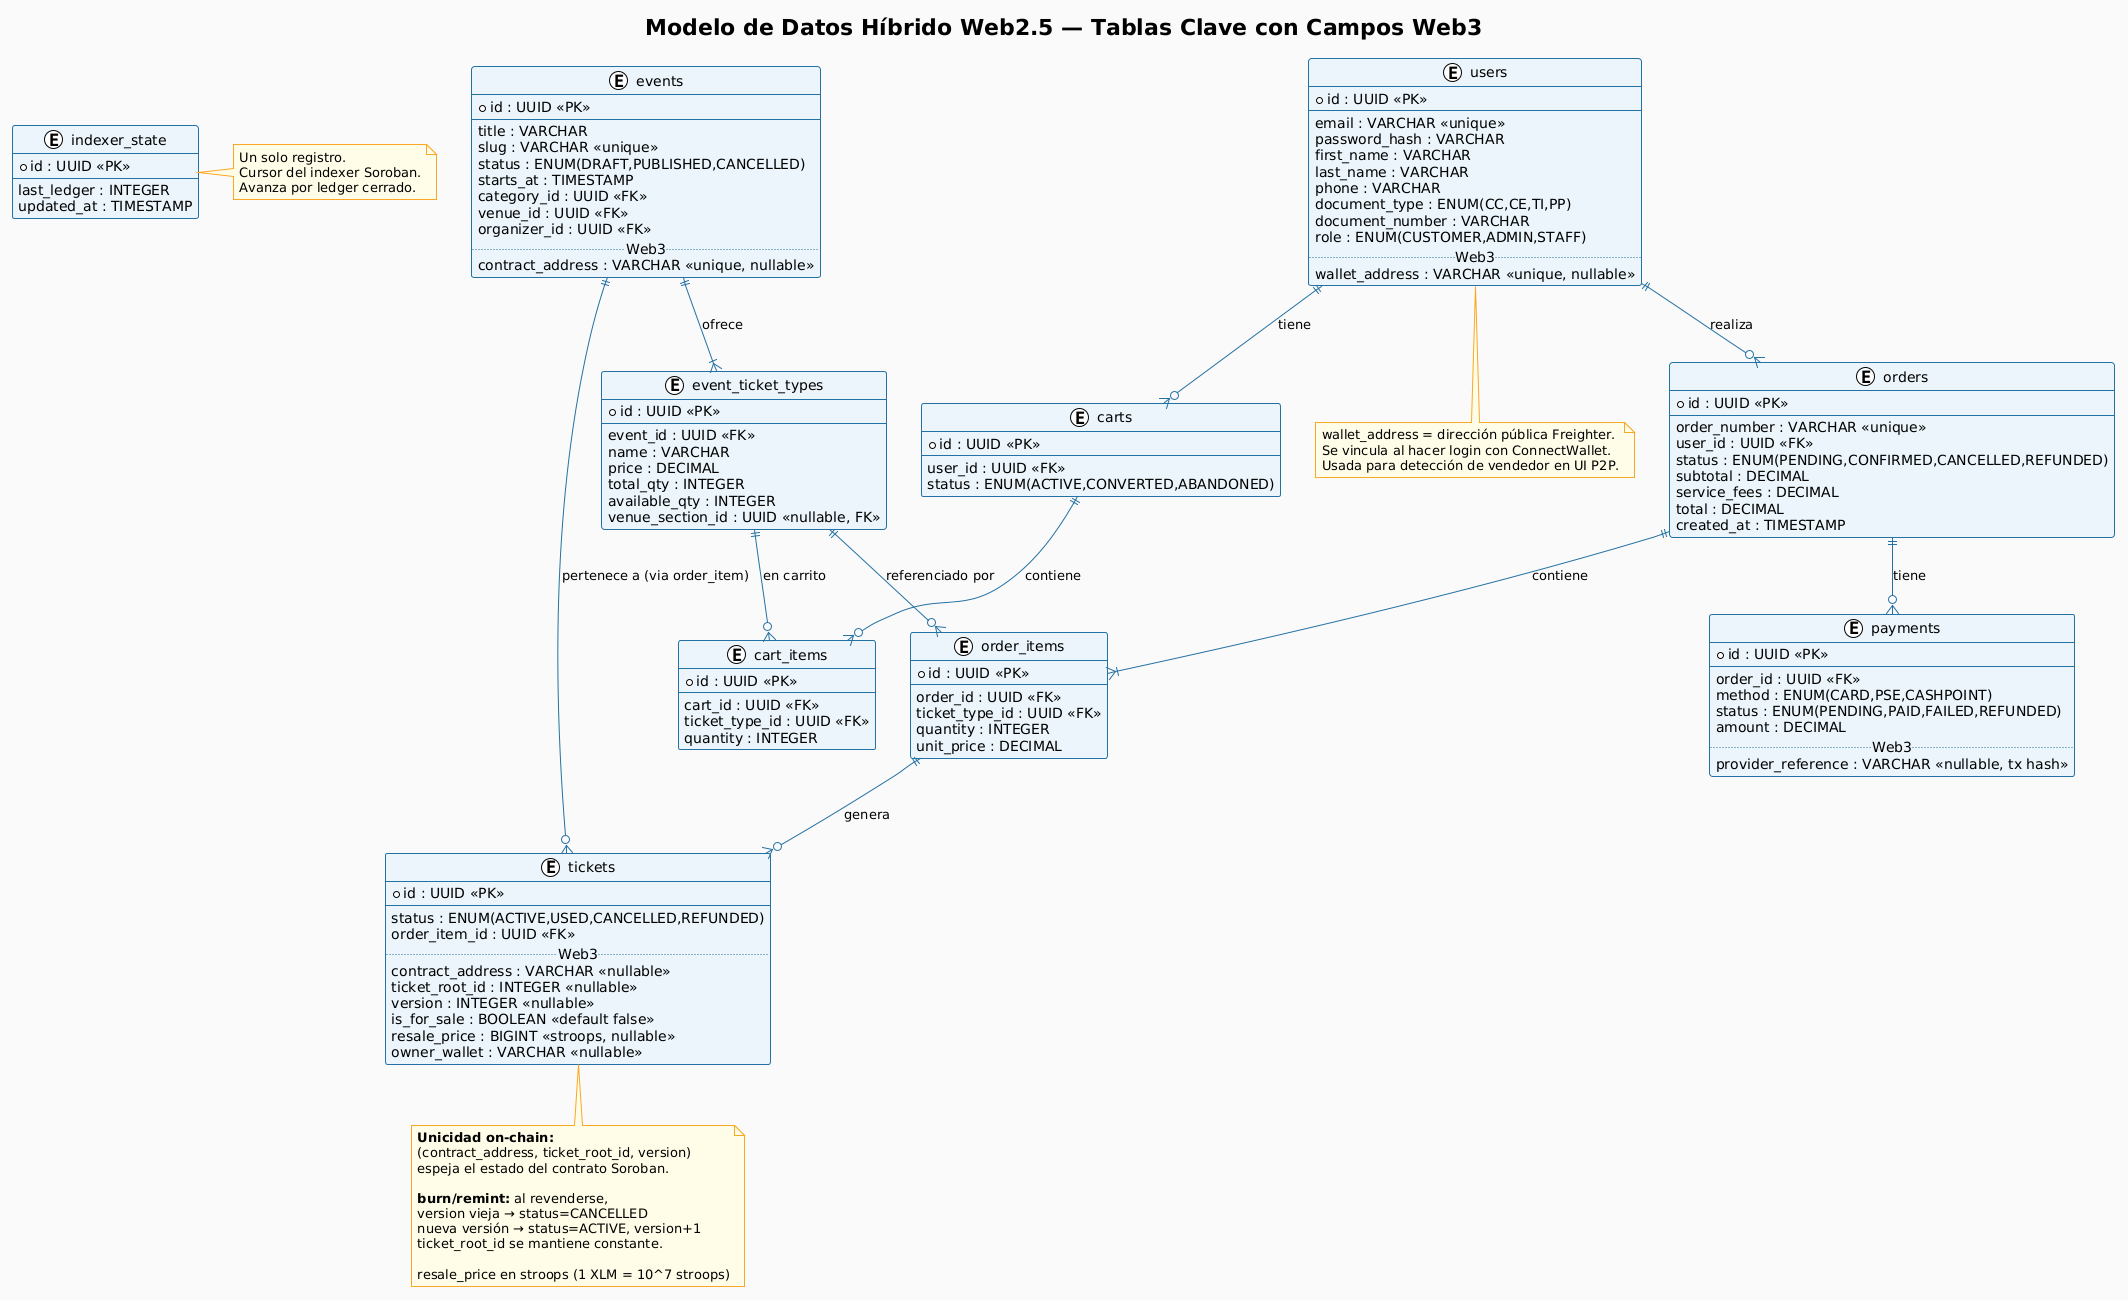
\includegraphics[width=\textwidth]{Imagenes/08_erd_datos.png}
\caption{Modelo entidad-relación de la base de datos relacional (esquema \texttt{ticketing}).}
\label{fig:erd}
\end{figure}

\subsection{Frontend web}

La aplicación se ejecuta sobre Vite y emplea TanStack Query para gestión de caché HTTP, Framer Motion para transiciones y shadcn/ui sobre Radix para componentes. La integración con la billetera usa \texttt{@stellar/freighter-api} 6.0.1, cuya interfaz devuelve \texttt{isConnected}, \texttt{address} y \texttt{signedTxXdr}. El estado global vive en \texttt{AppContext.tsx} y comprende usuario autenticado, JWT (en \texttt{localStorage.authToken}), carrito, órdenes, entradas adquiridas, ventas P2P y dirección de la billetera vinculada. La función \texttt{apiFetch<T>} centraliza las llamadas con \texttt{Bearer} automático.

El componente \texttt{ConnectWallet.tsx} se renderiza solo si el usuario está autenticado y lee la dirección desde el contexto persistente. El componente \texttt{TicketCard.tsx} expone los flujos ``Asegurar en Blockchain'' (\textit{mint} on-chain y emisión del coleccionable) y ``Revender NFT'' (precio en COP, vista previa en XLM vía CoinGecko con caché de 5 min).

\subsection{Despliegue distribuido}

El despliegue se realiza sobre tres infraestructuras independientes, conforme al diagrama de despliegue de la Figura~\ref{fig:despliegue}:

\begin{figure}[H]
\centering
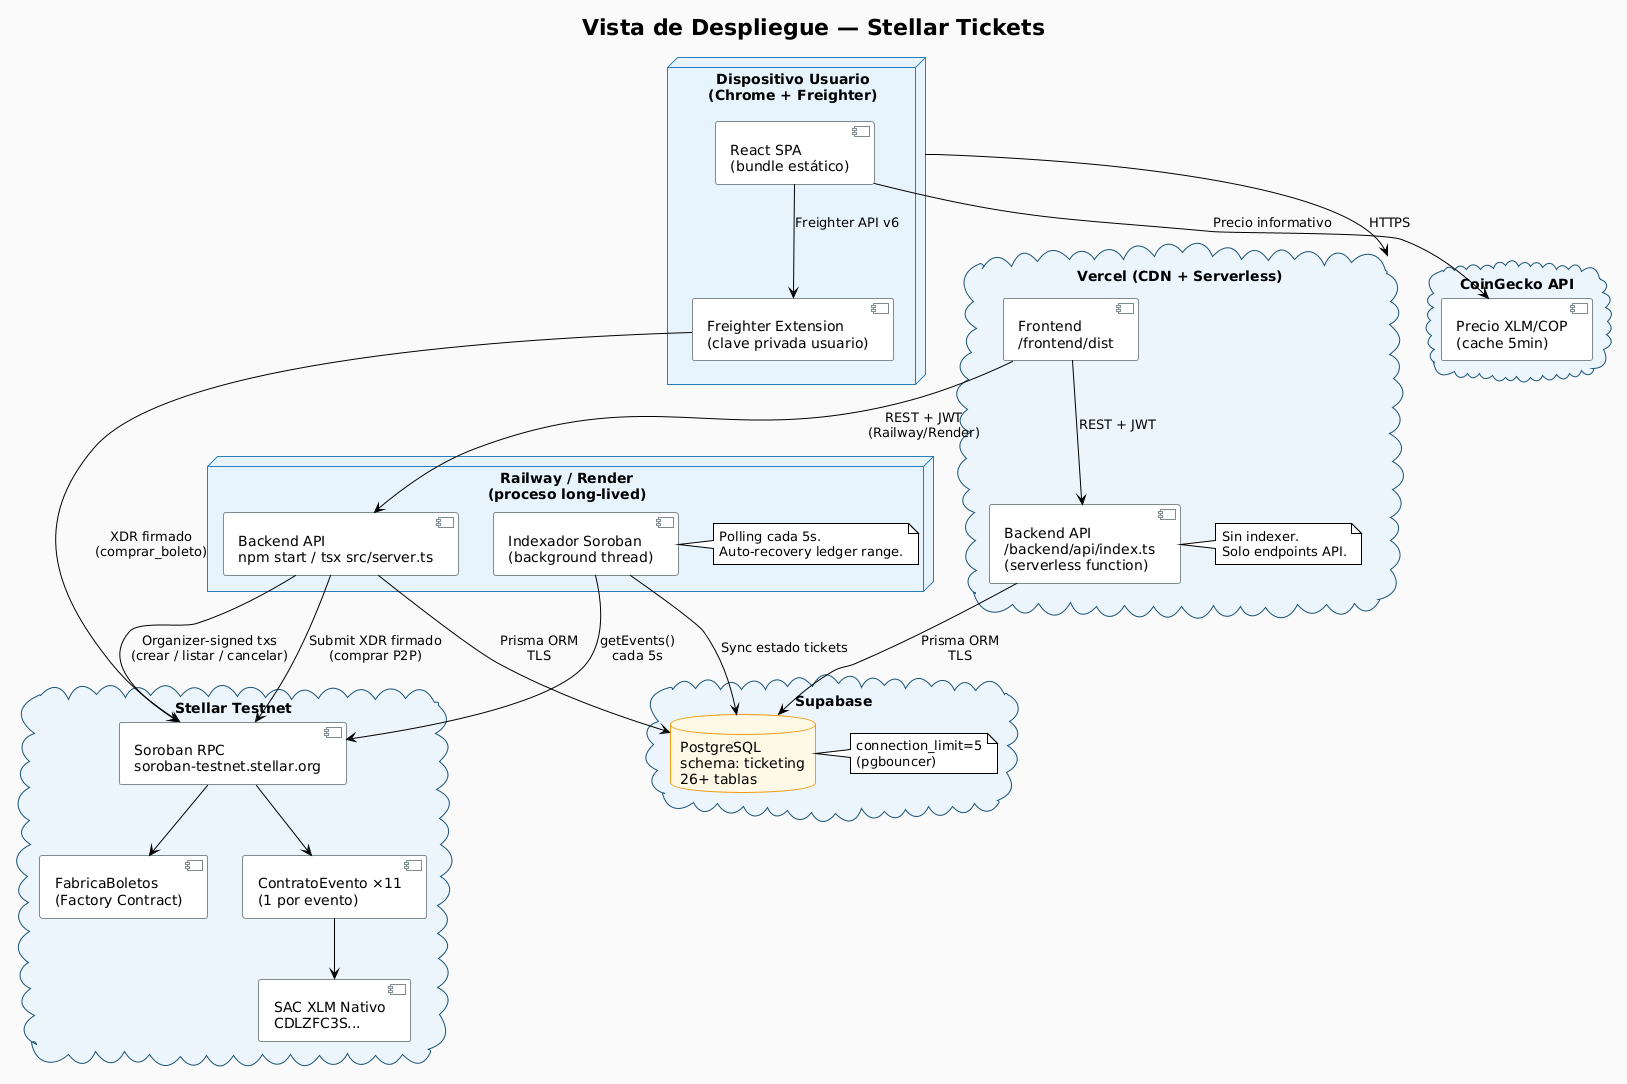
\includegraphics[width=\textwidth]{Imagenes/03_despliegue_produccion.png}
\caption{Diagrama de despliegue: frontend en Vercel, backend en Railway, base de datos PostgreSQL en Supabase y red Stellar testnet.}
\label{fig:despliegue}
\end{figure}

Los tres nodos físicos son:

\begin{itemize}\setlength{\itemsep}{2pt}
    \item \textbf{Frontend} en Vercel con \texttt{vercel.json} y reescrituras para el modelo SPA.
    \item \textbf{Backend} en Railway como servicio web persistente, necesario porque el indexador requiere ejecución continua en segundo plano.
    \item \textbf{Base de datos} PostgreSQL gestionada por Supabase, esquema \texttt{ticketing}, \texttt{connection\_limit=5}.
\end{itemize}

El despliegue de contratos en testnet se ejecuta mediante \texttt{backend/scripts/deploy-contracts.ts} y \texttt{deploy-nft-contracts.ts}: carga de \textit{keypairs} desde \texttt{.env.deploy}, financiación con \textit{friendbot}, carga del WASM al ledger, despliegue de un \texttt{event\_contract} y un \texttt{ticket\_nft\_contract} por evento mediante el \textit{factory} y el \textit{deployer} dedicado, invocación de \texttt{inicializar} con comisiones 5/3 y persistencia de las direcciones en \texttt{events.contract\_address} y \texttt{events.nft\_contract\_address}. Al cierre del trabajo hay doce eventos con su par de contratos desplegado bajo el \textit{factory} configurado.

\subsection{Integración continua}

El repositorio incluye un \textit{workflow} de GitHub Actions en \texttt{.github/workflows/soroban.yml} que se ejecuta en cada \textit{push} y \textit{pull request} contra \texttt{main}. Utiliza \texttt{cargo-binstall} para instalar \texttt{stellar-cli} sin compilación desde fuentes, compila por paquete (\texttt{--package event\_contract}, \texttt{--package factory\_contract}, \texttt{--package ticket\_nft\_contract}) para evitar colisiones de símbolos en el target \texttt{wasm32v1-none}, ejecuta \texttt{cargo test} y publica el módulo WASM como artefacto. Esta automatización constituye la evidencia operacional de la trazabilidad de cambios sobre el código fuente.

\subsection{Pruebas}

La estrategia se organiza en cuatro niveles: (i) \textit{pruebas unitarias} sobre contratos, 58 casos cubriendo ciclo de vida, precondiciones, 16 errores tipados, doble autenticación del \textit{factory} y emisión/transferencia/quema del NFT; (ii) \textit{pruebas de integración} E2E que cubren registro, navegación, compra fiat, ``Asegurar en Blockchain'', listado, compra de reventa con Freighter, redención y cancelación; (iii) \textit{pruebas antifraude} con escenarios negativos (doble redención, doble compra, autocompra, redención no autorizada, manipulación de precio); (iv) \textit{pruebas de medición} con captura de tiempos y costos sobre testnet, cuyos resultados alimentan la sección de Resultados.
